\section{Results}
\label{sec:results}

\subsection{Logit Lens Reveals a Non-Monotonic Information Trajectory}
\label{sec:results_logitlens}

\Figref{fig:logit_lens} shows the mean target probability $P^{(\ell)}(o)$ across all 24 layers. The trajectory is strikingly non-monotonic: factual information is absent in early layers (0--7), first emerges at layers 8--9, and fluctuates through layers 10--14 before entering a peak enrichment zone at layers 15--17. The absolute peak occurs at layer 21 ($P = 0.025$), after which probability \emph{decreases} to 0.009 at layer 23.

\begin{figure}[t]
    \centering
    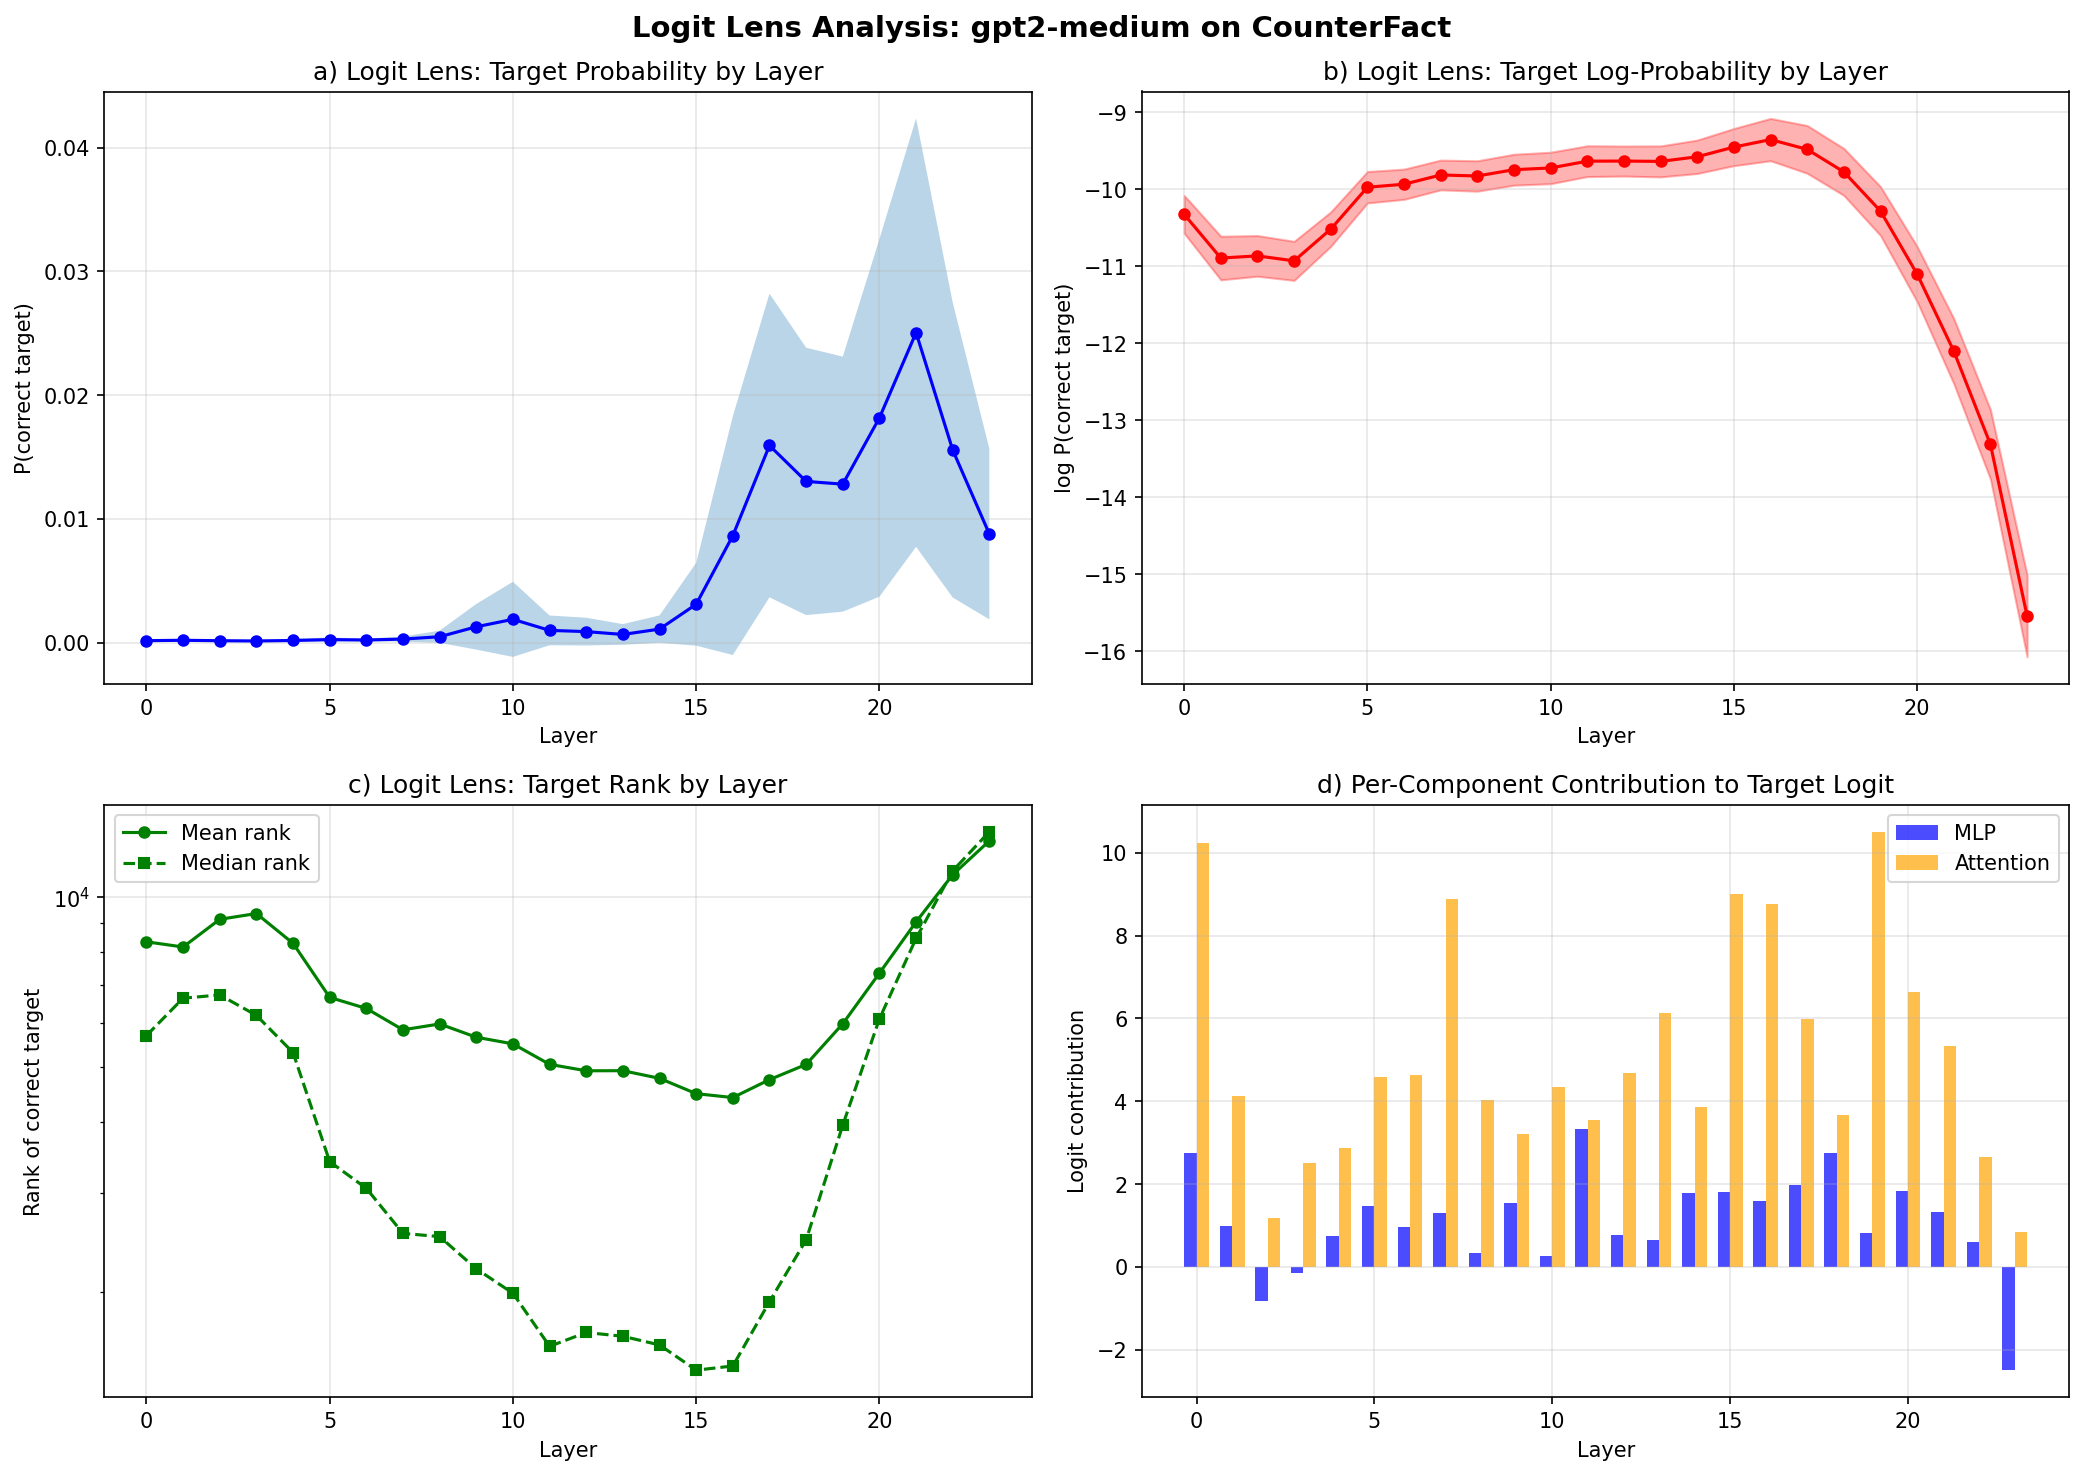
\includegraphics[width=0.95\linewidth]{figures/fig1_logit_lens_comprehensive.png}
    \caption{Logit lens profile across 24 layers of \gptmed, averaged over 200 \counterfact examples. \figleft Mean target probability $P^{(\ell)}(o)$, showing non-monotonic trajectory with peak at layer 21 followed by suppression. \figright Per-layer enrichment score $\Delta P^{(\ell)}$, highlighting the primary enrichment zones at layers 16--17 and 20--21, and the suppression zone at layers 22--23.}
    \label{fig:logit_lens}
\end{figure}

This non-monotonic pattern reveals \emph{natural information deletion}: the model actively suppresses factual signal in its final layers. The top three enrichment layers are 17 ($\Delta P = +0.0073$), 21 ($\Delta P = +0.0069$), and 16 ($\Delta P = +0.0055$). The suppression at layers 22--23 suggests that late computations redistribute probability mass away from the initially enriched target.

\para{MLP vs.\ attention contributions.} Attention heads dominate the target logit contribution at nearly every layer (mean 4.7 vs.\ 1.2 for MLPs). The largest attention contributions come from layers 0 (10.2), 7 (8.9), 15 (9.0), 19 (10.5), and 16 (8.8), consistent with a two-stage architecture where MLPs store knowledge and attention heads extract and route it.

\para{Per-fact variation.} The enrichment pattern is not uniform across facts (\figref{fig:heatmap}). Some facts show sharp enrichment at layers 8--9 while others emerge only at layer 16--17, suggesting that different facts are stored at different layers.

\begin{figure}[t]
    \centering
    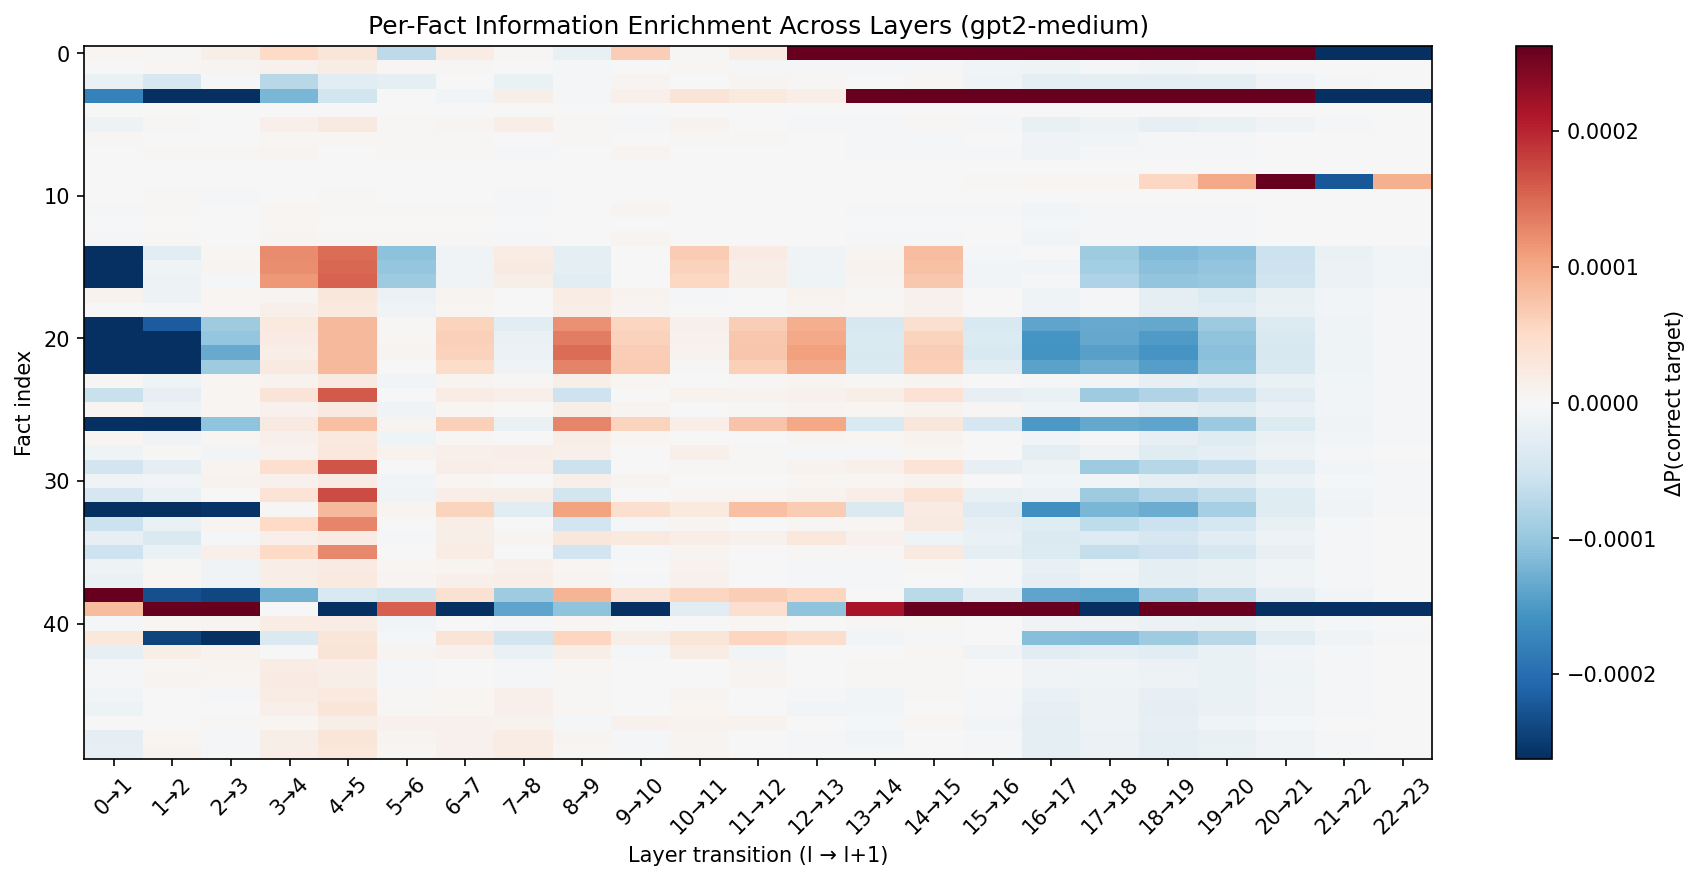
\includegraphics[width=0.95\linewidth]{figures/fig4_enrichment_heatmap.png}
    \caption{Per-fact enrichment heatmap showing $\Delta P^{(\ell)}$ for each of the 200 facts (rows) across layers (columns). While the population average peaks at layers 16--17 and 20--21, individual facts show diverse enrichment patterns, with some enriched as early as layer 8 and others only at layer 20.}
    \label{fig:heatmap}
\end{figure}

\subsection{Early MLPs Are the Critical Storage Components}
\label{sec:results_ablation}

\Figref{fig:ablation} and \tabref{tab:ablation} present the ablation results. MLP ablation reveals a clear hierarchy: layer 0 is the most critical ($\Delta P = 0.0087$, accounting for nearly 100\% of the baseline probability of 0.0088), followed by layers 6 ($\Delta P = 0.0036$) and 3 ($\Delta P = 0.0031$).

\begin{figure}[t]
    \centering
    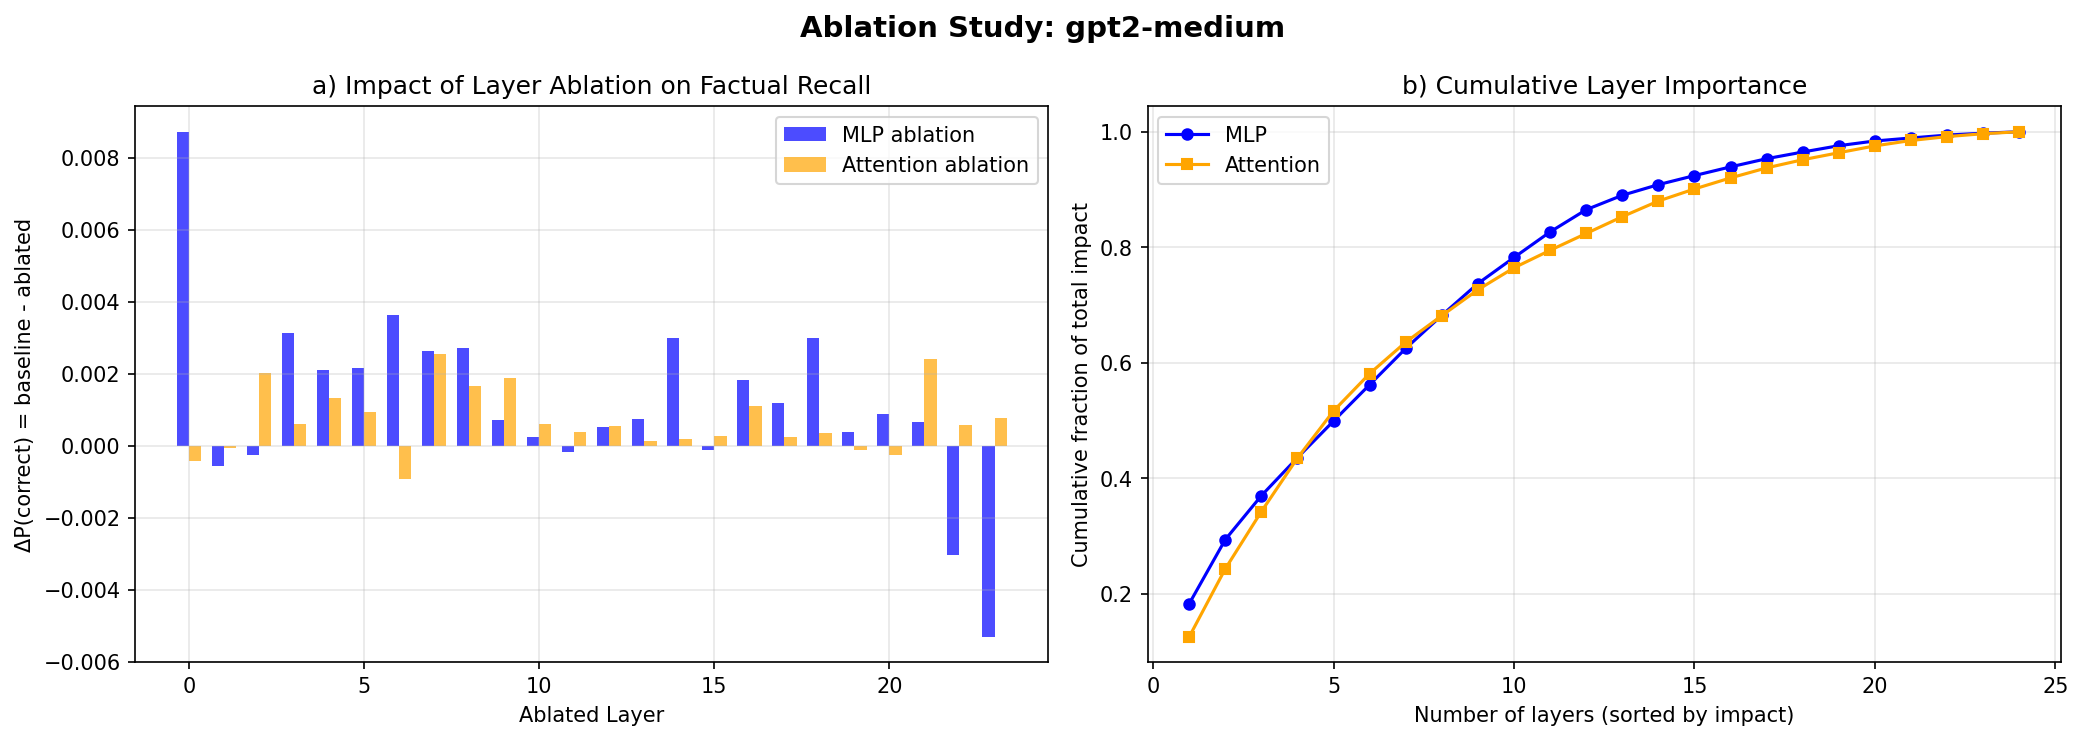
\includegraphics[width=0.95\linewidth]{figures/fig2_ablation_study.png}
    \caption{Impact of zero-ablating individual MLP and attention components on final-layer target probability. Early MLPs (layers 0, 3, 6) show the largest positive impact, while late MLPs (layers 22--23) show \emph{negative} impact---ablating them \emph{increases} recall, confirming their role in information suppression.}
    \label{fig:ablation}
\end{figure}

\begin{table}[t]
    \centering
    \caption{Top ablation impacts by component type. MLP ablation impact $\Delta P_{\text{MLP}}^{(\ell)}$ measures the drop in target probability when MLP$^{(\ell)}$ is zeroed; attention impact $\Delta P_{\text{Attn}}^{(\ell)}$ is analogous. Baseline mean $P(o) = 0.0088$. Bold indicates the most critical component per type.}
    \label{tab:ablation}
    \resizebox{\textwidth}{!}{%
    \begin{tabular}{@{}lcccccccc@{}}
        \toprule
        & \multicolumn{4}{c}{\textbf{Top MLP Layers}} & \multicolumn{4}{c}{\textbf{Top Attention Layers}} \\
        \cmidrule(lr){2-5} \cmidrule(lr){6-9}
        & Layer 0 & Layer 6 & Layer 3 & Layer 18 & Layer 7 & Layer 21 & Layer 19 & Layer 2 \\
        \midrule
        $\Delta P$ & {\bf 0.0087} & 0.0036 & 0.0031 & 0.0030 & {\bf 0.0026} & 0.0024 & 0.0010 & 0.0006 \\
        \% of baseline & {\bf 98.9\%} & 40.9\% & 35.2\% & 34.1\% & {\bf 29.5\%} & 27.3\% & 11.4\% & 6.8\% \\
        \bottomrule
    \end{tabular}%
    }
\end{table}

Late MLPs (layers 22, 23) have \emph{negative} ablation impact: zeroing them \emph{increases} target probability. This confirms that late MLPs participate in the information suppression observed in the logit lens trajectory (\secref{sec:results_logitlens}).

\subsection{Directional Deletion Achieves Near-Complete Knowledge Removal}
\label{sec:results_deletion}

\Tabref{tab:deletion} summarizes the directional deletion results. Projecting out the mean fact direction at layer 0 alone reduces target probability by 90.2\% (from $5.3 \times 10^{-3}$ to $5.0 \times 10^{-4}$). Adding layer 3 achieves 99.7\% reduction ($1.4 \times 10^{-5}$); adding layer 6 provides no further benefit, confirming that the critical factual signal is concentrated in the two earliest MLPs.

\begin{table}[t]
    \centering
    \caption{Directional deletion results. We project out the mean fact direction from MLP outputs at the specified layers and measure the reduction in target probability. Effect sizes (Cohen's $d$) and $p$-values are from paired $t$-tests across 200 facts.}
    \label{tab:deletion}
    \begin{tabular}{@{}lcccccc@{}}
        \toprule
        \textbf{Strategy} & \textbf{Layers} & \textbf{Pre-$P$} & \textbf{Post-$P$} & \textbf{Reduction} & \textbf{Cohen's $d$} & \textbf{$p$-value} \\
        \midrule
        Single best & $\{0\}$ & $5.3 \times 10^{-3}$ & $5.0 \times 10^{-4}$ & 90.2\% & 0.221 & 0.116 \\
        Top 2 & $\{0, 3\}$ & $5.3 \times 10^{-3}$ & $1.4 \times 10^{-5}$ & {\bf 99.7\%} & 0.245 & 0.088 \\
        All critical & $\{0, 3, 6\}$ & $5.3 \times 10^{-3}$ & $1.4 \times 10^{-5}$ & {\bf 99.7\%} & 0.245 & 0.088 \\
        \bottomrule
    \end{tabular}
\end{table}

\para{Statistical significance.} The $p$-values of 0.088--0.116 reflect marginal significance. The moderate values arise from high variance across facts---many have near-zero baseline probability---and the relatively small effective sample of well-recalled facts. The Cohen's $d$ values of 0.22--0.25 (small-to-medium) are typical for transformer interventions.

\subsection{Deletion Fundamentally Reshapes Residual Stream Geometry}
\label{sec:results_geometry}

\begin{figure}[t]
    \centering
    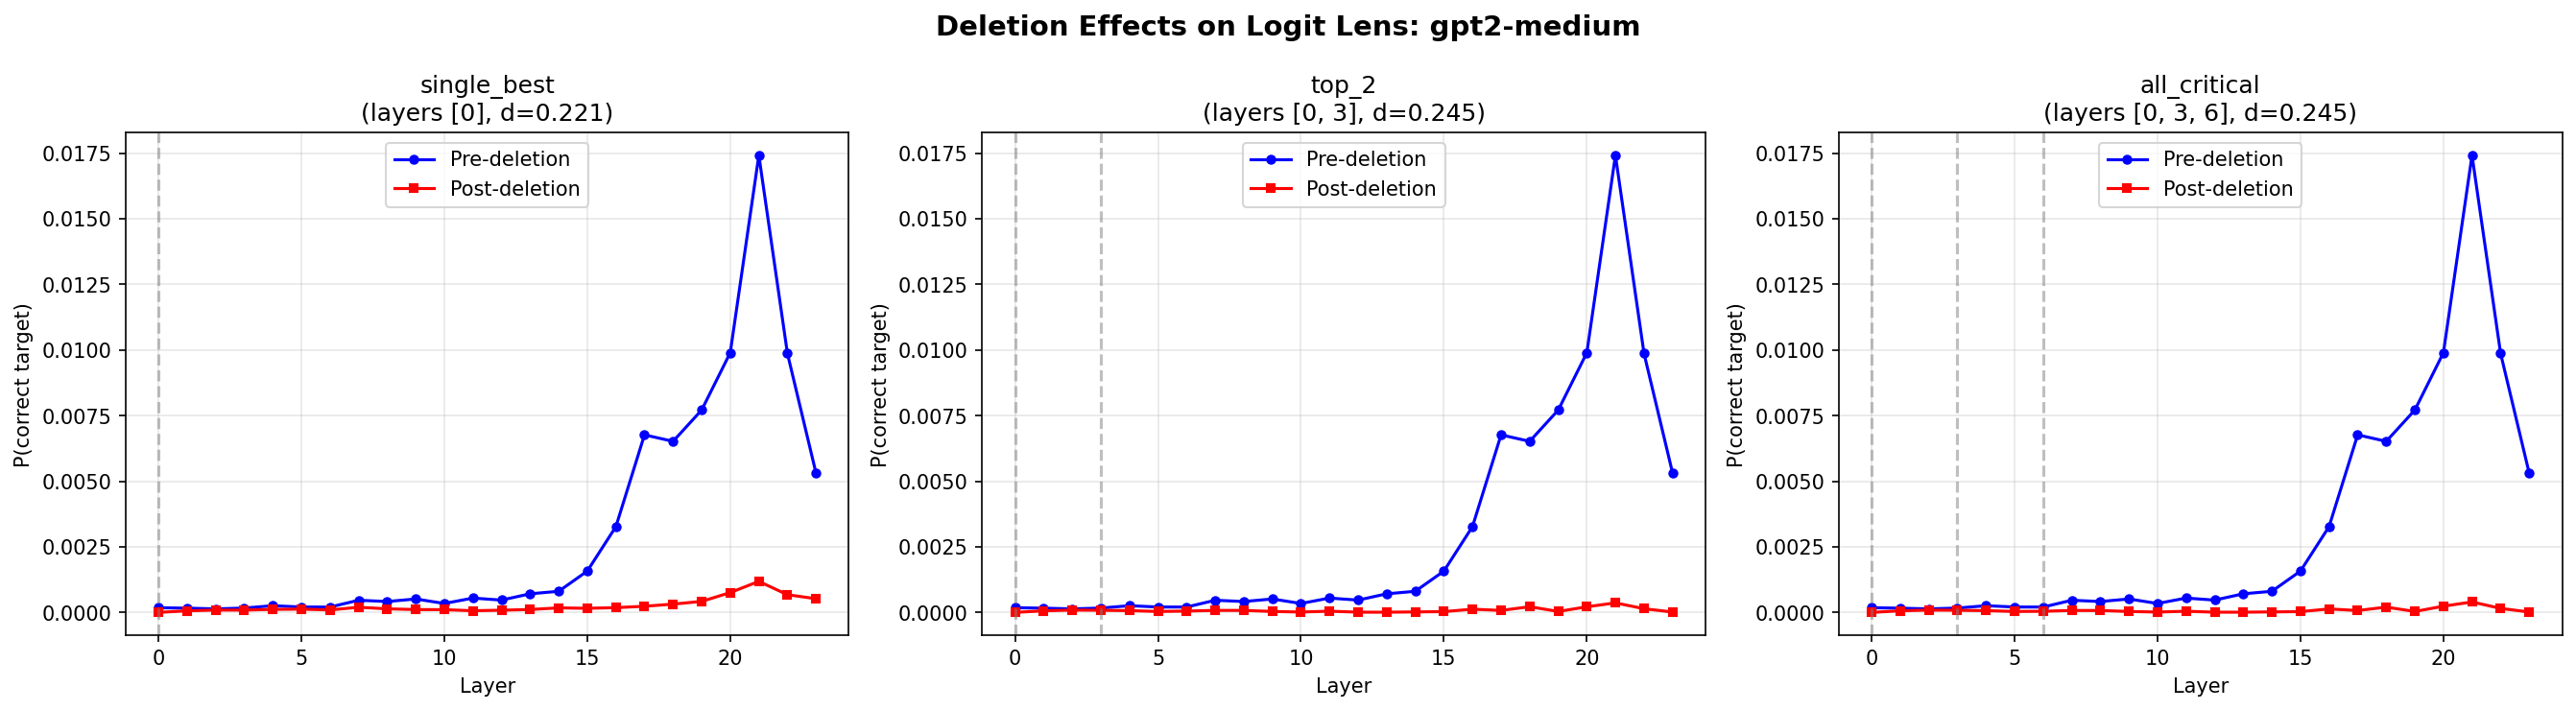
\includegraphics[width=0.95\linewidth]{figures/fig3_deletion_effects.png}
    \caption{Geometric impact of directional deletion. \figleft Cosine similarity between pre- and post-deletion activations at layers 0, 12, and 23 for single-layer and all-critical deletion strategies. Multi-layer deletion drives final-layer similarity to $\approx 0$. \figright $L_2$ distance between pre- and post-deletion activations, showing displacement exceeding the mean activation norm at the final layer.}
    \label{fig:deletion_geometry}
\end{figure}

The directional deletion has dramatic geometric consequences (\figref{fig:deletion_geometry} and \tabref{tab:geometry}). Single-layer deletion (layer 0 only) reduces cosine similarity at the targeted layer to 0.117 but allows substantial recovery by layer 23 (similarity 0.879). Multi-layer deletion (layers 0, 3, 6) prevents this recovery: final-layer cosine similarity drops to $-0.009$ (effectively zero), and the $L_2$ displacement reaches 1357.7---exceeding the mean activation norm at layer 23 (1055). The deletion pushes activations into a fundamentally different region of the \residstream.

\begin{table}[t]
    \centering
    \caption{Geometric impact of deletion at three measurement layers. Cosine similarity and $L_2$ distance are computed between pre- and post-deletion \residstream activations, averaged over 200 facts.}
    \label{tab:geometry}
    \begin{tabular}{@{}llcc@{}}
        \toprule
        \textbf{Layer} & \textbf{Strategy} & \textbf{Cosine Sim.} & \textbf{$L_2$ Distance} \\
        \midrule
        0  & Single best   & 0.117 & 128.3 \\
        12 & Single best   & 0.684 & 301.9 \\
        23 & Single best   & 0.879 & 501.5 \\
        \midrule
        0  & All critical  & 0.117 & 128.3 \\
        12 & All critical  & 0.623 & 330.4 \\
        23 & All critical  & {\bf $-$0.009} & {\bf 1357.7} \\
        \bottomrule
    \end{tabular}
\end{table}

\subsection{Geometric Structure of the Residual Stream}
\label{sec:results_pca}

\begin{figure}[t]
    \centering
    \begin{subfigure}[t]{0.32\textwidth}
        \centering
        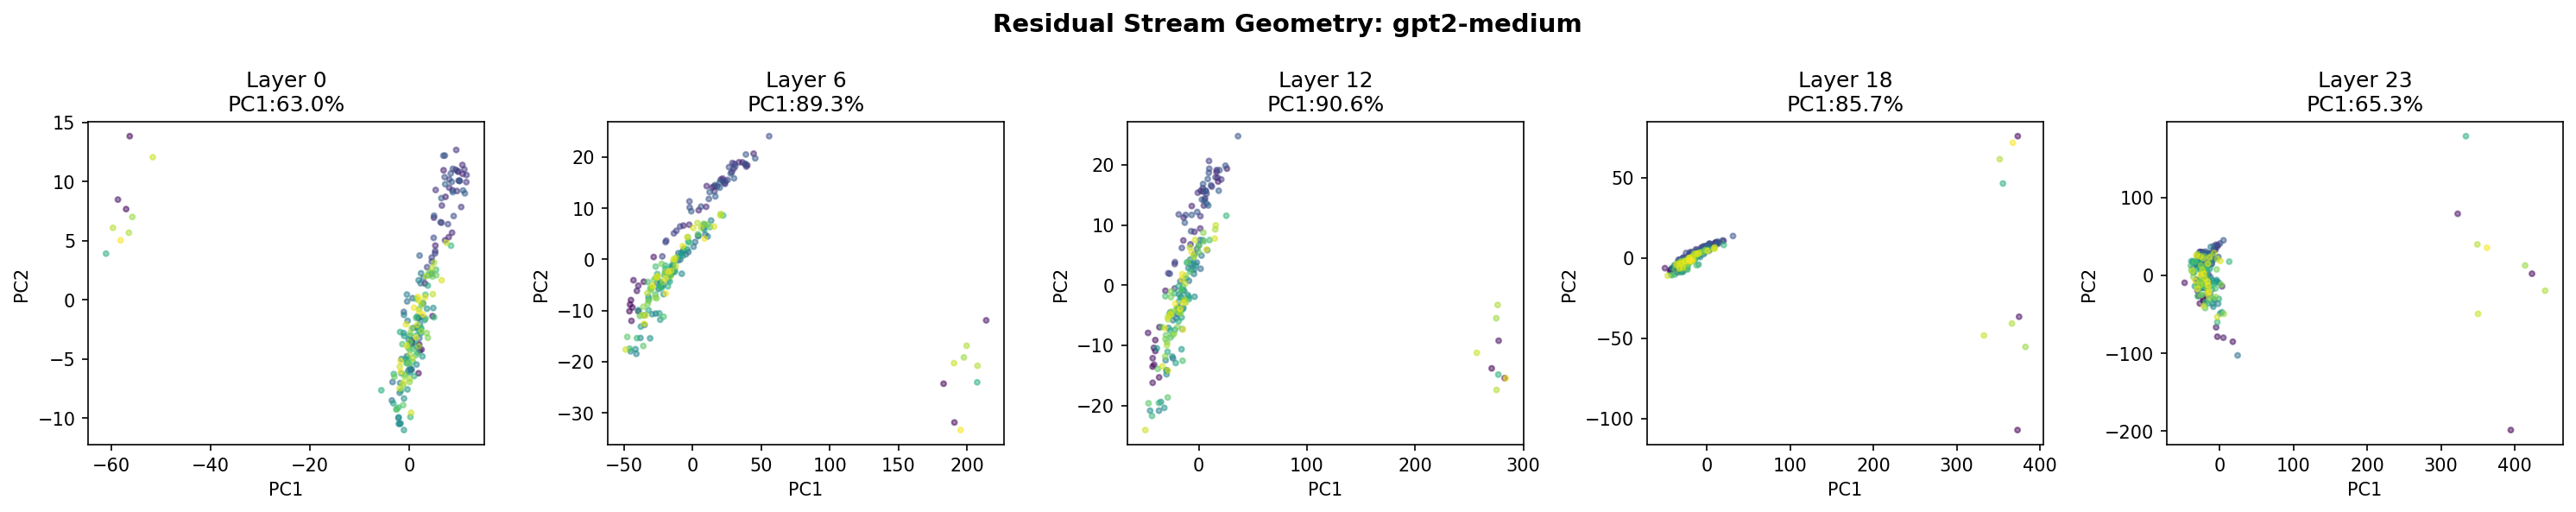
\includegraphics[width=\linewidth]{figures/fig5_geometry_pca.png}
        \caption{PCA variance explained}
        \label{fig:pca}
    \end{subfigure}
    \hfill
    \begin{subfigure}[t]{0.32\textwidth}
        \centering
        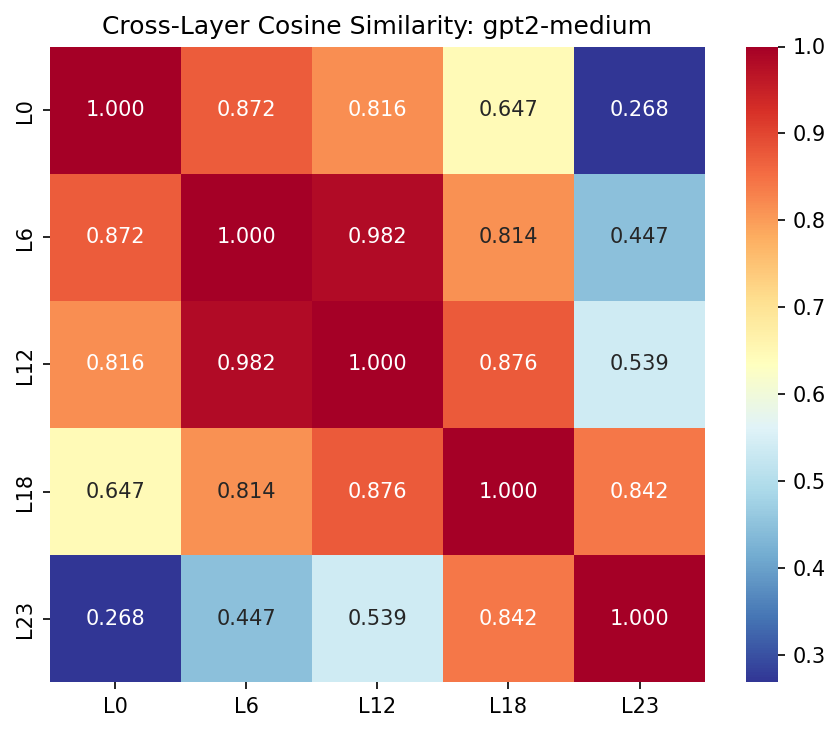
\includegraphics[width=\linewidth]{figures/fig6_cross_layer_similarity.png}
        \caption{Cross-layer cosine similarity}
        \label{fig:cross_layer}
    \end{subfigure}
    \hfill
    \begin{subfigure}[t]{0.32\textwidth}
        \centering
        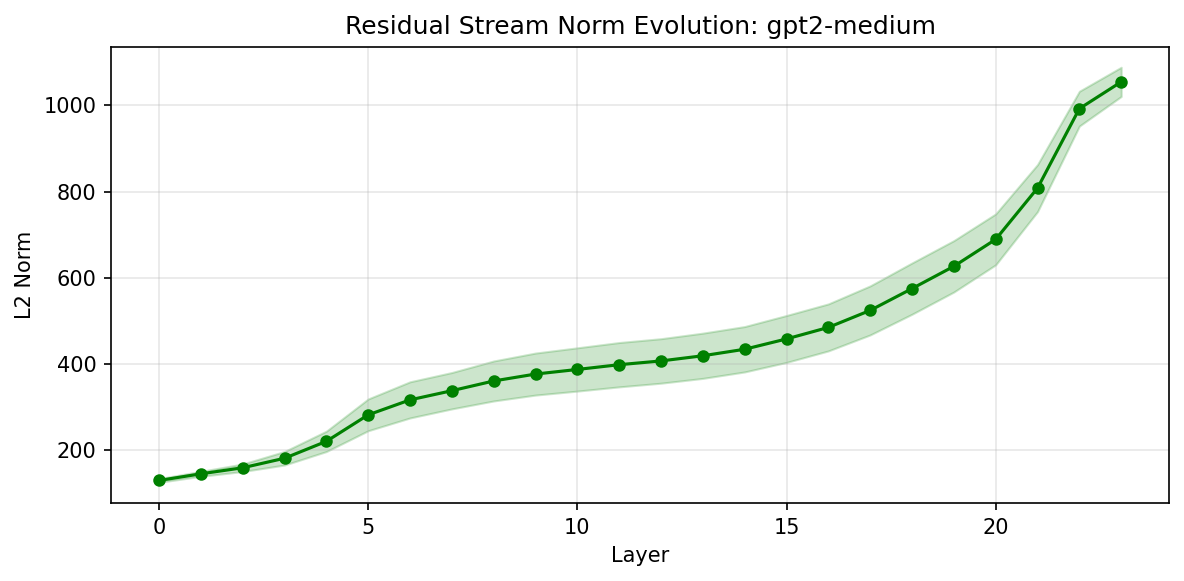
\includegraphics[width=\linewidth]{figures/fig7_norm_evolution.png}
        \caption{Norm evolution}
        \label{fig:norms}
    \end{subfigure}
    \caption{Geometric properties of the \residstream. \captiona The first principal component captures 63--91\% of variance, with peak dominance at middle layers. \captionb Cosine similarity drops sharply with layer distance, confirming substantial rotation across layers. \captionc $L_2$ norms grow monotonically from 130 (layer 0) to 1055 (layer 23), with accelerating growth in late layers.}
    \label{fig:geometry}
\end{figure}

The \residstream exhibits strong anisotropy at all layers (\tabref{tab:pca}). A single principal component captures 63.0\% of variance at layer 0, rising to 90.6\% at layer 12, before decreasing to 65.3\% at layer 23. This dominant direction---a ``rogue dimension''~\citep{belrose2023tuned}---is most prominent in middle layers and becomes less dominant at the output, possibly reflecting the need to support a diverse vocabulary distribution.

\begin{table}[t]
    \centering
    \caption{PCA variance explained at selected layers. The \residstream is dominated by a single principal component at all layers, with peak anisotropy in middle layers (6--12).}
    \label{tab:pca}
    \begin{tabular}{@{}lccc@{}}
        \toprule
        \textbf{Layer} & \textbf{PC1 Var. (\%)} & \textbf{PC2 Var. (\%)} & \textbf{Top-10 Cum. (\%)} \\
        \midrule
        0  & 63.0 & 14.7 & 95.4 \\
        6  & 89.3 & 4.4  & 98.9 \\
        12 & {\bf 90.6} & 2.7  & 99.4 \\
        18 & 85.7 & 2.8  & 99.4 \\
        23 & 65.3 & 10.0 & 98.0 \\
        \bottomrule
    \end{tabular}
\end{table}

Activation norms grow monotonically from 130 at layer 0 to 1055 at layer 23 (\figref{fig:norms}), with particularly rapid growth in late layers (808 at layer 21 $\to$ 993 at layer 22 $\to$ 1055 at layer 23). This exponential growth means that a fixed-magnitude perturbation has proportionally less impact at later layers---a geometric constraint on the effectiveness of late-layer interventions.

Cross-layer cosine similarity (\figref{fig:cross_layer}) drops sharply with distance: adjacent layers maintain high similarity ($>0.85$), while distant pairs (\eg layer 0 vs.\ 23) show low similarity ($\sim$0.20). The \residstream undergoes substantial rotation across layers, implying that information encoded in early layers may be geometrically distant from the same information as represented in late layers.
